\section{9/17/2019}

\subsection{Outline}

The \nameref{def:mdf} enjoys strong robustness bounds such
as \myref{prop:mdf-modulus-error-bound}. However, its definition
involves performing a projection onto $\cG$ (the set of distributions which
$p^*$ is assumed to be contained in):
\begin{align}
  \hat\theta(\tilde{p}) &= \theta^*(q) = \min_\theta L(q,\theta)
  \text{ where }q = \argmin_{q \in \cG} D(\tilde{p}, q)
\end{align}
We saw last time $D=\TV$ was not suitable if $\tilde{p} = \tilde{p}_n$ is discrete,
motivating the use of \nameref{def:tilde-tv}.
For bounded $k$th moments, we have that $\rho = \cO(\sigma_k \eps^{1 - 1/k})$
which under our previous theory (\cref{prop:mdf-tilde-tv} and \cref{eq:9-12-desidirata-2})
yields a guarantee
\begin{align}
  \|\mu(\tilde{p}_n) - \mu(p^*)\|_2 \leq \cO\left( \left(\underbrace{\eps + \sqrt{\frac{d}{n}}}_{\eps'}\right)^{1 - 1/k}\right)
\end{align}
whenever $\widetilde{\TV}_{\cH_{lin}}(\tilde{p}, p^*) \leq \eps$.

Today, we consider an alternative solution where we expand $\cG$ to some
larger set $\cM$ to perform the projection:
\begin{align}
  q = \argmin_{q \in \cM} \tilde{D}(\tilde{p}, q)
\end{align}
Under this analysis, we can achieve a tighter $\cO\left(\eps^{1 - 1/k} + \sqrt{d/n}\right)$ error.

Outline for today:
\begin{itemize}
  \item True ``empirical distribution''
  \item Expand the set idea
  \item Analyze concentration for bounded $k$th moments
    \begin{itemize}
      \item symmetrization
      \item truncated moments
      \item ledoux-talagrand
    \end{itemize}
\end{itemize}

\subsection{True Empirical Distribution}

Let $p_n^*$ define an empirical distribution drawn from $p^*$.

\begin{figure}[H]
\begin{center}
  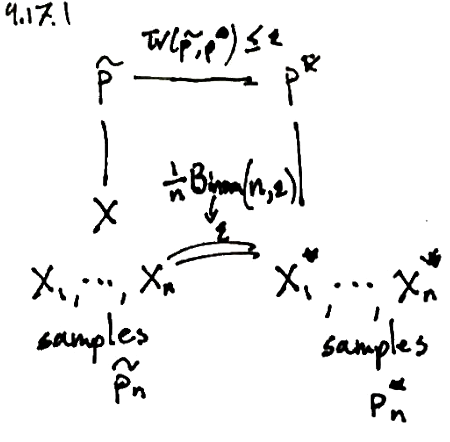
\includegraphics[width=0.3\textwidth]{figures/9-17-1.png}
\end{center}
\end{figure}


\textbf{Issue}: No overlap between $\tilde{p}_n$, $p_n^*$

\textbf{Solution}: Define \emph{coupling} between $p_n^*$ and $\tilde{p}_n$.

\begin{figure}[H]
\begin{center}
  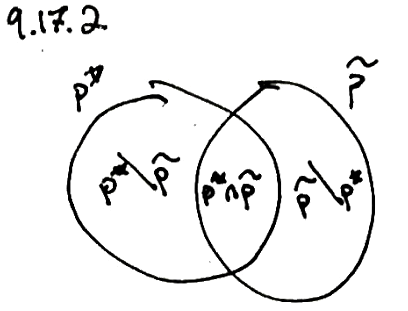
\includegraphics[width=0.3\textwidth]{figures/9-17-2.png}
\end{center}
\end{figure}

\begin{itemize}
  \item
    With probability $1 - \eps$:
    \begin{itemize}
      \item Sample from $p^* \cap \tilde{p}$, $X_i = \tilde{X_i} =$ sample
    \end{itemize}
  \item
    And with probability $\eps$:
    \begin{itemize}
      \item Sample $X_i^*$ from $p^* \setminus \tilde{p}$
      \item Sample $X_i$ from $\tilde{p} \setminus p^*$
    \end{itemize}
\end{itemize}

\textbf{Takeaway}:
$\underbrace{\TV(\tilde{p}_n, p_n^*)}_{\tilde{\eps}} \sim \frac{1}{n}\text{Binom}(n, \eps)$

\begin{lemma}[Tail bound for binomials]
  With probability $\geq 1 - \delta$
  \begin{align}
    \frac{1}{n} \text{Binom}(n, \eps)
    \leq O\left(\sqrt{\eps} + \sqrt{\frac{\log \frac{1}{\delta}}{2 n}}\right)^2
    = O\left(\eps + \frac{\log \frac{1}{\delta}}{2 n}\right)
  \end{align}
\end{lemma}

\begin{remark}
  This is tighter than Hoeffding, which would have given $\exp(-\eps^2 n / 3)$.
  Need Bernstein's inequality and Chernoff bound for binomial random variables
  to prove this.
\end{remark}

\subsection{Finite-Sample Concentration via Expanding the Set}%

\begin{figure}[H]
  \begin{center}
    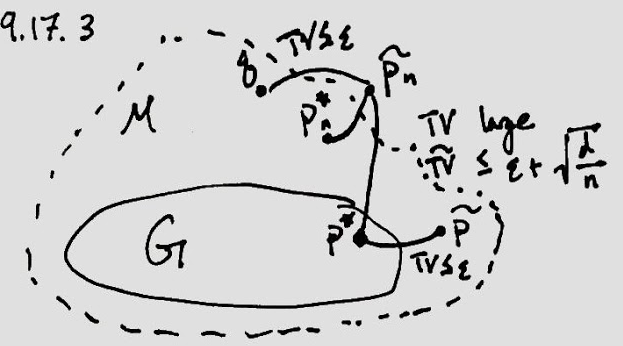
\includegraphics[width=0.5\textwidth]{figures/9-17-3.png}
    \caption{If we can expand $\cG \subset \cM$ so that $p_n^* \in \cM$,
      then we can form $q = \min_{q \in \cM} \TV(\tilde{p}_n, q)$ by projecting
      $\tilde{p}_n$ onto $\cM$ and use the ``true empirical distribution'' $p_n^*$
      to connect $q$ with $p^*$. This is made precise in \cref{prop:projection-bound-expand-G-to-M}}
  \end{center}
\end{figure}

Need three properties for $\cM$
\begin{itemize}
  \item $\cM$ large: $p_n^* \in \cM$ whp.
  \item $\cM$ small: modulus $\fm(\cM_{\eps})$ small
  \item $p_n^*$ good approx to $p^*$: $\|\mu(p^*) - \mu(p_n^*)\|_2$ bounded
\end{itemize}

\begin{proposition}\label{prop:projection-bound-expand-G-to-M}
  Suppose
  \begin{itemize}
    \item $p^*_n \in \cM$ wp $1 - \delta$
    \item $\TV(p_n^*, \tilde{p}_n) \leq \tilde{\eps}$ wp $1 - \delta$
  \end{itemize}
  Then projecting onto $\cM$ yields $q$ where
  \begin{align}
    \|\mu(q) - \mu(p^*)\|_2 \leq \fm(\cM, 2 \tilde{\eps}) + \|\mu(p^*) - \mu(p_n^*)\|_2
  \end{align}
  wp $1 - 2 \delta$.
\end{proposition}

\begin{proof}
  Since $p_n^* \in \cM$, we have
  \begin{align}
    \TV(\tilde{p}_n, q) &= \min_{q \in \cM} \TV(\tilde{p}_n, q) \leq \tilde{\eps}
  \end{align}
  Also by hypothesis $\TV(\tilde{p}_n, p_n^*) \leq \tilde{\eps}$, so
  by triangle inequality
  \begin{align}
    \TV(p_n^*, q) \leq 2 \tilde{\eps}
  \end{align}
  Together we have $\|\mu(p_n^*) - \mu(q)\|_2 \leq \fm(\cM, 2\tilde{\eps})$
  and by triangle inequality
  \begin{align}
    \|\mu(p^*) - \mu(q)\|_2 \leq \fm(\cM, 2 \tilde{\eps}) + \|\mu(p^*) - \mu(p_n^*)\|_2
  \end{align}
\end{proof}

\subsection{Expanding bounded kth moments to set of resilient distributions}

The following example will be our running example for this section.
We will see how bounded $k$th moments may require $n$ to be too large, and how
we can expand to the larger set of resilient distributions.

\begin{example}[Bounded $k$th moments]
  Consider distributions with bounded $k$th moments, that is
  \begin{align}
    \cG = \cG_k(\sigma)
    &= \{ p : \lvert \ex X \rvert_{\psi_k} \leq \sigma \} \\
    &= \{ p : \ex_p[ \lvert \braket{X - \mu, v} \rvert^k] \leq \sigma_k^k~\forall \|v\|_2 \leq 1\}
  \end{align}
  where $\psi_k(x) = x^k$.
  For example, $\cG_2(\sigma)$ are the distributions with bounded covariance.

  \textbf{Isuse}: $p_n^* \not\in \cG$ until $n \gg d^{k/2}$. For example,
  let $p^* = \cN(\mu, I)$, $p_n^* = \sum_{i=1}^n \frac{1}{n} \delta_{x_i}$,
  and notice for $v = \frac{x_1 - \mu}{\|x_1 - \mu\|}$
  we have $\|v\|_2 = 1$ but
  \begin{align}
    \ex_{p_n^*}[\lvert \braket{X - \mu, v}\rvert^k]
    \geq \frac{1}{n} \lvert \braket{x_1 - \mu, v}\rvert^k
    = \frac{1}{n} \underbrace{\|X_1 - \mu\|_2^k}_{=\cO(\sqrt{d})}
    &\asymp \frac{1}{n} d^{k/2} \\
    \ex_{p_n^*}[\lvert \braket{X - \mu, v}\rvert^k]^{1/k}
    &\asymp \left( \frac{1}{n} d^{k/2} \right)^{1/k}
    = \frac{\sqrt{d}}{n^{1/k}}
  \end{align}
  Asymptotically, we see that we need $n \gg d^{k/2}$ for the $k$th moments to
  remain bounded.

  \begin{figure}[H]
    \begin{center}
      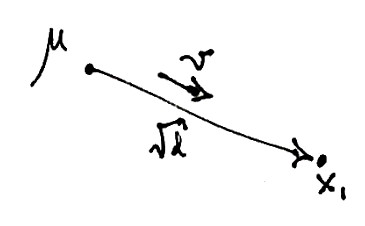
\includegraphics[width=0.3\textwidth]{figures/9-17-4.png}
    \end{center}
    \caption{The moment $\braket{X - \mu, v}$ along a
      single direction of a sample $v = \frac{x_1 - \mu}{\|x_1 - \mu\|}$
      is large, need to average over many samples before it washes out.}
  \end{figure}
\end{example}

Consider expanding bounded $k$th moments $\cG = \cG_k(\sigma)$ to the larger
set of resilient distributions $\cM = \cG_{\TV}(\rho, \eps)$ with $\rho = O(\eps^{1 - 1/k})$.
We already have a modulus bound $\fm(\cM, \eps) \leq 2 \rho = O(\eps^{1 - 1/k})$
from \myref{corr:mod-bound-resilient}, so
to make \cref{prop:projection-bound-expand-G-to-M} meaningful
it remains to show:
\begin{itemize}
  \item Bound 
    $\|\mu(p^*) - \mu(p_n^*)\|_2 = O\left(\sigma \sqrt{\frac{d}{n} \delta^{-1/k}}\right)$
    We do this using Kintchine's inequality.

  \item $p^*_n \in \cM$ whp. 
    We do this using truncated moments.
\end{itemize}

\begin{lemma}
  \begin{align}
    \|X\|_2 &= \ex_{v \sim \cN(0,I)}[\lvert\braket{x,v}\rvert] \sqrt{\frac{\pi}{2}}
  \end{align}
\end{lemma}
\begin{proof}
  \begin{align}
    \ex[\lvert
    \braket{
      (\|x\|_2, 0, \ldots, 0),
      (v_1,\ldots, v_d)
    } \rvert]
    = \ex[\lvert v_1 \rvert \cdot \|x\|_2] \\
    \ex[\lvert v_1\rvert] = \sqrt{2/\pi}
  \end{align}
\end{proof}

\begin{remark}
  There's a better version of the above called \emph{Khintchine's inequality}:
  \begin{align}
    \|X\|_2 \leq \sqrt{2} \ex[\lvert \braket{X, \eps} \rvert]
  \end{align}
  with $\eps \sim \text{Rad}$. So we can just test using Rademachers rather
  than Gaussian process.
\end{remark}

\todo{We failed to prove the second easy thing in class using above, see next lecture for resolution}

\subsubsection{Truncated moments}

Now we show $p_n^* \in \cM$, introducing some new ideas along the way.

\textbf{Problem}: $\| \cdot \|_{\psi_k}$ is not small.

\textbf{Solution}: Truncate moments, replace $\psi_k(x) = x^k$ with
\begin{align}
  \tilde{\psi}_k(x) = \begin{cases}
    x^k & x \leq x_0 \\
    k x_0^{k-1} (x - x_0) + x_0^k & x > x_0
  \end{cases}
\end{align}
This is equal to $\psi_k$ for $x \leq x_0$ and linearly interpolates beyond $x \geq x_0$.

\begin{figure}[H]
  \begin{center}
    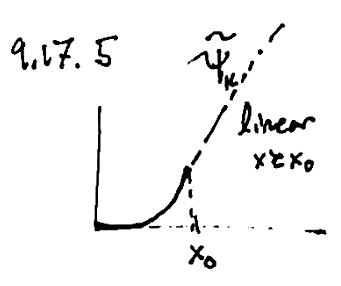
\includegraphics[width=0.3\textwidth]{figures/9-17-5.png}
  \end{center}
  \caption{The Orlicz function $\tilde{\psi}_k$ used for truncating moments}
  \label{fig:tilde-psi-k}
\end{figure}

$\tilde{\psi}_k$ is $L$-Lipschitz with $L = k x_0^{k-1}$, so in particular
if we choose $x_0 = \left(\frac{1}{\eps}\right)^{1/k}$ then we have $L = k / \eps^{1 - 1/k}$.

\begin{proposition}\label{prop:truncated-moments-bound}
  Let $X_1, \ldots, X_n \sim p^*$, where $p^* \in \cG_k(\sigma)$. Then
  \begin{align}
    \ex_{X_i \sim p^*}\left[
      \sup_{\|u\|_2 = 1} \frac{1}{n} \sum_{i=1}^n \tilde{\psi}_k\left(
        \left\lvert \frac{\braket{X_i - \mu, v}}{\sigma}\right\rvert
      \right)
    \right]
    &\leq 1 + 2 L \sqrt{\frac{d}{n}}
  \end{align}
  where $L = k x_0^{k-1}$.
\end{proposition}

\begin{remark}
  When  $n \geq 4 L^2 d = 4 k^2 d / \eps^{2 - 2/k}$, we have
  \begin{align}
    \sup_{\|u\|_2 = 1} \frac{1}{n} \sum_{i=1}^n \tilde{\psi}_k\left(
      \left\lvert \frac{\braket{X_i - \mu, v}}{\sigma}\right\rvert
    \right)
    \leq 2
  \end{align}
  This implies that $p_n^*$ has bounded Orlicz norm
  $\|p_n^*\|_{\tilde{\psi}_k}$, so by \cref{lem:orlicz-norm-resilient}
  $p_n^*$ is resilient with parameter $\sigma \eps \tilde{\psi}^{-1}(2/\eps)$.
  So we really need to control how fast $\sigma \eps \tilde{\psi}^{-1}(2/\eps)$
  grows. From \cref{fig:bound-tilde-psi-k-inv}, we may conclude
  \begin{align}
    \sigma \eps \tilde{\psi}^{-1}(2/\eps)
    \leq 2 \sigma \eps \underbrace{\left(\frac{1}{\eps}\right)^{1/k}}_{> 0}
    = 2 \sigma \eps^{1 - 1/k}
  \end{align}


  \begin{figure}[H]
    \begin{center}
      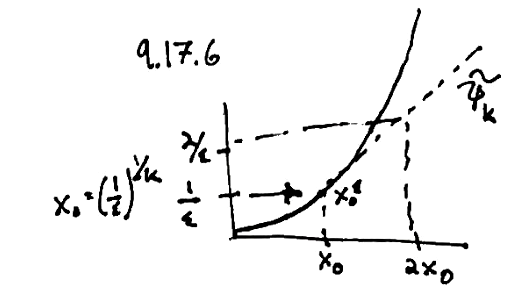
\includegraphics[width=0.4\textwidth]{figures/9-17-6.png}
    \end{center}
    \caption{A proof by picture why $\psi^{-1}(2/\eps) \leq 2 x_0 = 2 \eps^{-1/k}$}
    \label{fig:bound-tilde-psi-k-inv}
  \end{figure}

\end{remark}

\subsubsection{Ledoux-Talagrand contraction}%
\label{ssec:ledoux-talagrand-first}

This result is used as part of symmetrization arguments. If I have already symmetrized and I have
a Lipschitz function, than I can always repalce the function with just its
arguments and make things bigger.

\begin{theorem}[Ledoux-Talagrand]
  \begin{align}
    \ex_{\eps}\left[
      \sup_{v \in V} \frac{1}{n} \sum^{n}_{i=1} \eps_i \phi(\braket{x_i, v})
    \right]
    \leq \ex_\eps\left[
      \sup_{v \in V} \frac{1}{n} \sum_{i=1}^n \eps_i \braket{x_i, v}
    \right]
  \end{align}
  for $\phi$ $1$-Lipschitz, i.e. $\vert \phi(x) - \phi(y) \rvert \leq \lvert x - y \rvert$,
  $V$ a symmetric set, and $\eps \sim \text{Rad}$.
\end{theorem}

\begin{proof}[Proof of \cref{prop:truncated-moments-bound}]
  \begin{align}
    \ex_{X_i \sim p^*}\left[
      \sup_{\|u\|_2 = 1} \frac{1}{n} \sum_{i=1}^n \tilde{\psi}_k\left(
        \left\lvert \frac{\braket{X_i - \mu, v}}{\sigma}\right\rvert
      \right)
    \right]
    = \underbrace{\ex[\tilde{\psi}]}_{\leq \ex\psi \leq 1} + \sup_{\|v\|_2 \leq 1} \frac{1}{n} \sum^{n}_{i=1} \left(
      \tilde{\psi}_k(\lvert \braket{x_i - \mu, v} / \sigma \rvert) - \ex[\tilde\psi]
    \right)
  \end{align}

  Symmetrize?
  \begin{align}
    \ex_{X_i, X_i' \sim p^*, \eps \sim \text{Rad}}\left[
      \sup_{\|v\|_2 \leq 1} \frac{1}{n} \sum^{n}_{i=1}
      \eps_i \left(
        \tilde{\psi}_k\left(\frac{\lvert \braket{X_i - \mu, v}\rvert}{\sigma}\right)
        -  \tilde{\psi}_k\left(\frac{\lvert \braket{X_i' - \mu, v}\rvert}{\sigma}\right)
      \right)
    \right]
  \end{align}
  \todo{See next lecture}
\end{proof}
